%% JTEOH: Copied from the ACM template on overleaf, along with relevant files. I commented out irrelevant sections such as ISBN, Copyright, DOI.

%%%% Proceedings format for most of ACM conferences (with the exceptions listed below) and all ICPS volumes.
\documentclass[sigconf]{acmart}

% jteoh: Remove conference information. Courtesy of https://tex.stackexchange.com/questions/346292/how-to-remove-conference-information-from-the-acm-2017-sigconf-template
\settopmatter{printacmref=false} % Removes citation information below abstract
\renewcommand\footnotetextcopyrightpermission[1]{} % removes footnote with conference information in first column
\pagestyle{plain} % removes running headers

%%%% As of March 2017, [siggraph] is no longer used. Please use sigconf (above) for SIGGRAPH conferences.

%%%% Proceedings format for SIGPLAN conferences 
% \documentclass[sigplan, anonymous, review]{acmart}

%%%% Proceedings format for SIGCHI conferences
% \documentclass[sigchi, review]{acmart}

%%%% To use the SIGCHI extended abstract template, please visit
% https://www.overleaf.com/read/zzzfqvkmrfzn


\usepackage{booktabs} % For formal tables
\usepackage{xspace}
\usepackage{listings}



% \usepackage[colorlinks=true, allcolors=blue]{hyperref} %option clash of some sort that I don't understand, so commented out. I think it's because of acmart.cls?



\newcommand{\todo}[1]{\textcolor{blue}{{\sf TODO}: #1}}
% Added jteoh for comment attribution (might not be a full TODO task)
\newcommand{\jteoh}[1]{\textcolor{red}{{\sf JT}: #1}}
\newcommand\tab[1][1cm]{\hspace*{#1}}
\newcommand{\pyex}{{\sc PyExZ3}\xspace}
\newcommand{\tool}{{\sc PyFinder}\xspace}
\newcommand{\pyexheader}{PyExZ3\xspace}
\newcommand{\toolheader}{PyFinder\xspace}

\newcommand{\codestmt}[1]{{\tt #1}}



% Copyright
%\setcopyright{none}
%\setcopyright{acmcopyright}
%\setcopyright{acmlicensed}
\setcopyright{rightsretained}
%\setcopyright{usgov}
%\setcopyright{usgovmixed}
%\setcopyright{cagov}
%\setcopyright{cagovmixed}


% DOI
% \acmDOI{10.475/123_4}

% ISBN
% \acmISBN{123-4567-24-567/08/06}

%Conference
% \acmConference[WOODSTOCK'97]{ACM Woodstock conference}{July 1997}{El
%   Paso, Texas USA}
% \acmYear{1997}
% \copyrightyear{2016}


% \acmArticle{4}
% \acmPrice{15.00}

% These commands are optional
%\acmBooktitle{Transactions of the ACM Woodstock conference}
% \editor{Jennifer B. Sartor}
% \editor{Theo D'Hondt}
% \editor{Wolfgang De Meuter}


\begin{document}
\title{Self-Attentive Classification Network \\ for Sentiment Analysis on Yelp Reviews}
% \titlenote{Produces the permission block, and
%   copyright information}
% \subtitle{Extended Abstract}
% \subtitlenote{The full version of the author's guide is available as
%   \texttt{acmart.pdf} document}


\author{Jonathan Hurwitz}
\affiliation{
  \institution{University of California, Los Angeles}
}
\email{hurwitz@cs.ucla.edu}



% The default list of authors is too long for headers.
% \renewcommand{\shortauthors}{B. Trovato et al.}


\begin{abstract}
Yelp is widely used for finding quality food and well respected store-front businesses. Yelp encourages users to write reviews by offering a "Yelp elite" program, where selected special users get discounts at restaurants. This paper studies the effectiveness of a self-attentive classification network on predicting the star rating of a Yelp review based solely on the text. Baselines were established using random forest classifier and single layer neural network models with average pooling on the word embeddings.
\end{abstract}

%
% The code below should be generated by the tool at
% http://dl.acm.org/ccs.cfm
% Please copy and paste the code instead of the example below.
%
% \begin{CCSXML}
% <ccs2012>
%  <concept>
%   <concept_id>10010520.10010553.10010562</concept_id>
%   <concept_desc>Computer systems organization~Embedded systems</concept_desc>
%   <concept_significance>500</concept_significance>
%  </concept>
%  <concept>
%   <concept_id>10010520.10010575.10010755</concept_id>
%   <concept_desc>Computer systems organization~Redundancy</concept_desc>
%   <concept_significance>300</concept_significance>
%  </concept>
%  <concept>
%   <concept_id>10010520.10010553.10010554</concept_id>
%   <concept_desc>Computer systems organization~Robotics</concept_desc>
%   <concept_significance>100</concept_significance>
%  </concept>
%  <concept>
%   <concept_id>10003033.10003083.10003095</concept_id>
%   <concept_desc>Networks~Network reliability</concept_desc>
%   <concept_significance>100</concept_significance>
%  </concept>
% </ccs2012>
% \end{CCSXML}

% \ccsdesc[500]{Computer systems organization~Embedded systems}
% \ccsdesc[300]{Computer systems organization~Redundancy}
% \ccsdesc{Computer systems organization~Robotics}
% \ccsdesc[100]{Networks~Network reliability}


% \keywords{ACM proceedings, \LaTeX, text tagging}


\maketitle

\section{Introduction}
Yelp is an American internet company that enables users to crowd-source review data for businesses. It's primarily used for restaurants, but other storefront-type businesses exist on the site as well. Yelp reviews are structured in the form of a text response with a star rating, as well as some optional photos. Readers typically use a business' star rating as a signal of the business' quality. In fact, it has been shown empirically by \cite{luca_2011} that a one-star increase led to a 59\% increase in revenue of restaurants. 

\par
Due to the sheer amount of readable text in the corpus of aggregated review data, it's unlikely that a typical reader would read all reviews in depth. The star rating is a much faster indicator of aggregated quality, but it is also a faster indicator at the review-level granularity. Readers often skim the review text but pay extra attention to the star rating that the reviewer has assigned. Yelp allows users to assign integer-valued star ratings between one and five. This complicates the free-market signaling process as there is inherent ambiguity between subsets. For example, 1 star and 2 star ratings are both bad, but the difference is not immediately clear. Similarly, 4 and 5 star ratings are both good, but analysis of reviews that garner 4 and 5 star ratings shows dramatic similarity. Oftentimes, a 4 star rating has text that is so positive it could be a 5 star rating. This ambiguity results in potentially inaccurate signals to readers, as a reviewer's text may be overwhelmingly positive yet their star rating may be sub-par. The opposite is also possible: a reviewer's text may be negative but the star rating is positive. Here is an example of a 3-star review with super negative sentiment:
\begin{quote}
	"I never write reviews.  But then I went to Armando's and felt the need to share.   I had a breakfast burrito, and i'll admit it was good until an uneasy feeling hit my stomach a couple hours later.  Food poisoning.   One of the worst experiences of my life.   Even my dog, who sniffs her own shit couldn't stand to be around me for 2 days.   I will never go back to this place."
\end{quote}
This could easily be a 1 star review. While the text is indicative of the issues with Armando's, quick readers will only be looking at star ratings, both individual and aggregate. Since this star rating is inaccurate, it is a misguiding market signal.
\par 
The approach discussed in this paper is based on the assumption that the majority of reviewers are rational, and that there is an implicit "mean" bijection between a reviewer's sentiment and a star rating. Concretely, the belief is that the majority of reviewers will think similarly. For example, an overwhelmingly positive review would be 5 star. A super negative review such as the one discussed above would be 1 star. The ratings in between are harder to accurately map. The aim is to learn this bijection by learning the underlying text features that correspond to more or less positive ratings. Labels consist of the star ratings, and the assumption of a mean bijection is used to justify the acceptance of outliers in the data. The model will take review input as text and output its predicted star rating. This mapping could be used to suggest a star rating to a user based on the sentiment and features of their text prior to posting a review. If the assumption were that yelp reviewers are irrational, then some method of transfer learning would be appropriate in order to preserve a text sentiment to integer output class bijection.

\par 
Additionally, there were several objectives defined after understanding the dataset breakdown. There were two datasets used, a severely imbalanced one from kaggle and a perfectly balanced one. 
These datasets are further explained in the following section. Additional project goals were defined as follows:
\begin{itemize}
	\item Effectively deal with a class imbalance.
	\item Study the effects of pre-trained word embeddings vs. embeddings trained at each training step.
	\item Use part-of-speech (POS) tags as an additional feature.
\end{itemize}

\section{Dataset}
Two datasets were used to study different aspects of the problem. 
\subsection{RecSys2013 Dataset}
The first dataset dataset was sourced from the yelp-recsys2013 kaggle competition \cite{kaggle} and consists of 229,898 reviews. The data consists of over 10,000 businesses, 8,000 check-in sites, and 40,000 users. All reviews were sourced from the Phoenix, Arizona metropolitan area.

\par 
The actual RecSys2013 competition has different problem setup than the problem discussed here, and it was only used as a data source. In the original problem discussed on Kaggle, users were also tasked with being able to predict a business' star rating, but the testing setup was different. Rather than learning purely from the review text, this problem provides features including business details, user details, and check-in information. The testing set withholds the actual review text and only provides user and business information. Therefore, the RecSys2013 testing set is unsuitable for use in this project. Instead, the training set was separated into a train, test, and dev set. Each set is disjoint since unique businesses were partitioned into each set rather than having crossover.
% Please add the following required packages to your document preamble:
% \usepackage{booktabs}
\begin{table}[H]
	\begin{tabular}{@{}ll@{}}
		\toprule
		\textbf{Set} & \textbf{Number of Examples} \\ \midrule
		Train        & 166101                      \\
		Dev          & 29312                       \\
		Test         & 34485                       \\ \bottomrule
	\end{tabular}
\caption{Imbalanced dataset train, dev, and test breakdown.}
\end{table}

The total dataset has a severe class imbalance. As such, this dataset was used to see how effective an imbalance mitigation technique such as loss weighting would be. Shown below are the class labels and the number of examples with that label:
\begin{table}[H]
	\begin{tabular}{ll}
		\hline
		\textbf{Class} & \textbf{Number of Examples} \\ \hline
		1              & 17567                       \\
		2              & 20615                       \\
		3              & 35436                       \\
		4              & 79708                       \\
		5              & 76572                      
	\end{tabular}
\caption{Number of examples in each class.}
\end{table}
The histogram shown below illustrates this severe class imbalance, with 69.97\% of examples in classes 4 and 5.


\begin{figure}[H]
	%\centering
%	\captionsetup{justification=centering}
	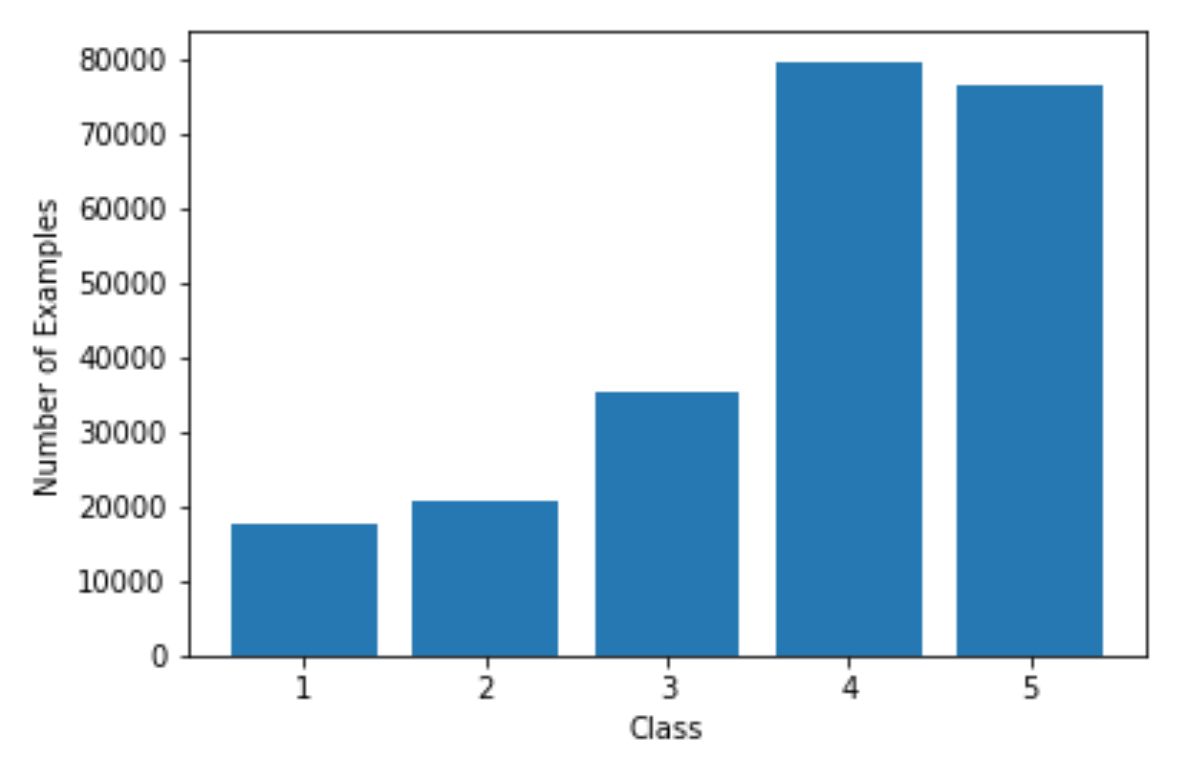
\includegraphics[width=0.5\textwidth]{images/recsys_balance.png}
	\caption{Class imbalance for the RecSys2013 dataset.}
\end{figure}

For the purposes of the RecSys2013 competition, this class imbalance was acceptable since the goal was not to predict a rating based on review text. Such a classifier trained on this dataset without any type of augmentation would result in memorization and outputting of the highest probability class. RecSys2013 involved other features, such as business characteristics and the actual user profiles in order to predict the ratings. Methods for dealing with such a class imbalanced are discussed in the models section.

\subsection{Balanced Dataset}
The other dataset was obtained from the authors of \cite{coneau_schwenk_lecun_barrault}. This dataset has 700,000 total reviews, and each class is perfectly balanced. Table \ref{tab:balancedbreakdown} shows the breakdown of train, test, and dev sets.
\begin{table}[H]
	\begin{tabular}{@{}ll@{}}
		\toprule
		\textbf{Set} & \textbf{Number of Examples} \\ \midrule
		Train        & 600000                      \\
		Dev          & 50000                       \\
		Test         & 50000                       \\ \bottomrule
	\end{tabular}
	\caption{\label{tab:balancedbreakdown}Balanced dataset train, dev, and test breakdown.}
\end{table}


%\footnote{\url{https://drive.google.com/drive/u/1/folders/0Bz8a_Dbh9Qhbfll6bVpmNUtUcFdjYmF2SEpmZUZUcVNiMUw1TWN6RDV3a0JHT3kxLVhVR2M}}
\section{Background}
In language, words are the building blocks upon which larger structures, such as phrases and sentences, are created. Words have inherent meanings based on their dictionary definitions, but their part of speech provides additional information into how the word can be used to assemble more complicated structures. Humans are very skilled at reading a sentence and determining the sentiment. The steps that occur behind the scenes include: per-word dictionary lookup for definition, linking from sequence (and subsequence) to other sequences (and subsequences) in order to form connections between subjects, objects, and actions, and finally special attention is paid to certain words such as adjectives, which help denote how someone is feeling about something. The first step to building a model that can emulate human sentiment analysis is to map a vocabulary of words to a continuous vector space that can be used as input to a model. This is referred to as word embeddings.  
\subsection{Word Embeddings}

Common word embedding methods include word2vec and GloVe \cite{pennington_socher_manning}. In the following discussions, GloVe pre-trained embeddings were used. Matrix factorization techniques such as latent semantic analysis (LSA) can capture global text statistics effectively but are deficient when it comes to actually capturing word to word meaning. GloVe combines matrix factorization with context. The GloVe method can be summarized as follows:
\begin{enumerate}
	\item Create a word co-occurrence matrix X. Some element $X_{ij}$ represents a count of how often word i appears in the context of word j. Context is determined by a window size before current term and after current term. In some instances, these may be two separate hyperparameters. Words that are closer are given higher weight and words that are farther are given lower weight with a penalty function:
	\begin{equation}
	penalty = \frac{1}{distance}
	\end{equation}
	\item Using ratios of co-occurrence probabilities rather than actual probabilities, create a model:
	\begin{equation}
	F(w_{i}, w_{j}, \tilde{w_{k}}) = \frac{P_{ik}}{P_{jk}}
	\end{equation}
	In this equation, $w \in R^d$ consist of word vectors and $\tilde{w} \in R^d$ is a context word vector. The next step is to formalize the definition of function F. Given a context k, we need to encode information regarding the probability ratio. Using linearity of the vector space we restrict the function F to a difference between the two words i and j that we care about:
	\begin{equation}
	F(w_{i} - w_{j}, \tilde{w_{k}}) = \frac{P_{ik}}{P_{jk}}
	\end{equation}
	Arguments on the left are vectors but the right hand side is a scalar. We take the dot product of the vector difference and the context, and enforce that F be a homomorphism as follows, in order to enforce labeling invariance:
	\begin{equation}
		F((w_{i} - w_{j})^T\tilde{w_{k}}) = \frac{F(w_{i}^T\tilde{w_{k}})}{F(w_{j}^T\tilde{w_k})}
	\end{equation}
	Numerator and denominator follow the same derivation, but the numerator on the right hand equates to $P_{ik}$, which is the co-occurrence of word i, context k, divided by count of word i. Concretely:
	\begin{equation}
	F(w_{i}^T\tilde{w_{k}}) = P_{ik} = \frac{X_{ik}}{X_{i}}
	\end{equation}
	Solving for the above equation by applying log to both sides:
	\begin{equation}
	w_{i}^T\tilde{w_{k}} = log(P_{ik}) = log(X_{ik}) - log(X_{i}) 
	\end{equation}
	The original paper moves the term $log(X_{i})$ into a bias term $b_{i}$ and rrearranges as follows:
	\begin{equation}
	w_{i}^T\tilde{w_{k}} + b_{i} + \tilde{b_{k}} = log(X_{ik})
	\end{equation}
	This equation has several problems. The logarithm diverges when $X_{ik}$ is zero. The simplest solution is to shift the function additively, but co-occurrences are still weighted equally. We want occurrences that are rare to not be underweighted and occurrences that are common not to be overweighted. Thus, a weighting function $f(X_{ij})$ is used as a coefficient in consideration of word i and word j's relation. 
	\item The cost function can be summarized as a least-squares problem given the weighting function:
	\begin{equation}
	J = \sum_{i,j=1}^{V}f(X_{ij})(w_{i}^T\tilde{w_{j}} + b_{i} + \tilde{b_{j}} - log(X_{ij}))^2
	\end{equation}
	The original authors chose the following weighting function to satisfy the expected requirements regarding divergence and appropriate weighting for rarity:
	\begin{equation}
	f(x)=\begin{cases}
	(\frac{x}{x_{max}})^\alpha, & \text{if $x<x_{max}$}.\\
	1, & \text{otherwise}.
	\end{cases}
	\end{equation}
\end{enumerate}


\subsection{LSTM}
Since text reviews consist of sequences of words, and sequences of larger hierarchical structures, it is appropriate to use models that can effectively learn sequence-to-sequence and chain dependencies. LSTMs are a class of RNN that solves some of the classic problems, namely the vanishing gradient problem in long-chain RNNs.
\par 
The LSTM can allow information to pass through easily, and can also add cell state regulated by gates. Each gate consists of a sigmoid activation and a pointwise multiplication. Smaller activations result in less information being let through, and vice versa. The overall LSTM architecture can be described as follows (images courtesy of Christopher Olah \cite{olah_2015}):
\begin{enumerate}
	\item Determine how much information to keep or forget from the cell state via a forget gate. This is a simgoid layer that considers current input as well as state of the previous time increment. Since the output is multiplied into the current cell state, output of 1 means that this information is kept, and zero means it is forgotten.
	\begin{equation}
	f_{t} = \sigma(W_{f}\cdot[h_{t-1}, x_{t}] + b_{f})
	\end{equation}
	Shown below is a figure illustrating the inputs for the forget gate:
	\begin{figure}[H]
		%\centering
		%	\captionsetup{justification=centering}
		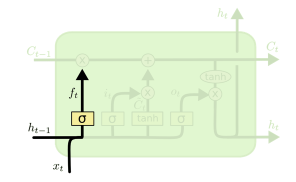
\includegraphics[width=0.5\textwidth]{images/LSTM_forget.png}
		\caption{LSTM cell forget gate.}
	\end{figure}

	\item Determine what information gets stored in teh cell states. The value ${i_{t}}$ is an input vector to the multiplication unit which determines which values are updated. It has the ability to zero-out entries. The $\tilde{C_{t}}$ vector consists of the entire set of candidate values to be added to the state. The multiplication unit combines these two.
	\begin{equation}
	i_{t} = \sigma(W_{i}\cdot[h_{t-1}, x_{t}] + b_{i})
	\end{equation}
	\begin{equation}
	\tilde{C_{t}} = tanh(W_{c}\cdot[h_{t-1}, x_{t}] + b_{C})
	\end{equation}
	\begin{figure}[H]
		%\centering
		%	\captionsetup{justification=centering}
		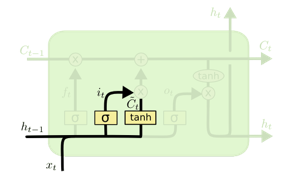
\includegraphics[width=0.5\textwidth]{images/LSTM_cell_input.png}
		\caption{LSTM cell input and candidate values.}
	\end{figure}

	\item Update the cell state. This is done by multiplication and addition blocks. First, the forget gate is multiplied by the cell state of the previous iteration in order keep and discard elements. The input selector vector is also multiplied by the candidate value vector to perform a state update:
	\begin{equation}
	C_{t} = f_{t}*C_{t-1} + i_{t}*\tilde{C_{t}}
	\end{equation}
	\begin{figure}[H]
		%\centering
		%	\captionsetup{justification=centering}
		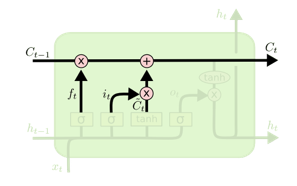
\includegraphics[width=0.5\textwidth]{images/LSTM_update.png}
		\caption{LSTM update cell state.}
	\end{figure}

	\item The final step involves passing current input and history multiplied by weights through another sigmoid activation to create a filtering vector. This vector is then multiplied by the tanh activation output of the current cell state in order to pick and choose which values contribute to the output, and to what degree:
	\begin{equation}
	o_{t} = \sigma(W_{o}[h_{t-1}, x_{t}] + b_{o})
	\end{equation}
	\begin{equation}
	h_{t} = o_{t}*tanh(C_{t})
	\end{equation}
	\begin{figure}[H]
		%\centering
		%	\captionsetup{justification=centering}
		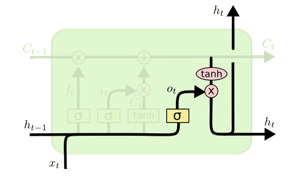
\includegraphics[width=0.5\textwidth]{images/LSTM_output.png}
		\caption{LSTM output.}
	\end{figure}

\end{enumerate}



%\begin{figure}
% \centering
% \captionsetup{justification=centering}
%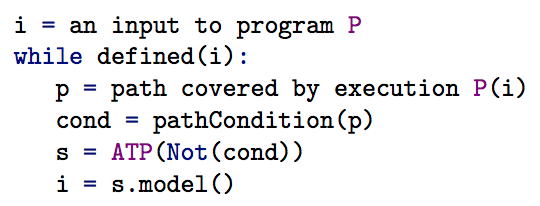
\includegraphics[width=0.5\textwidth]{images/dse_pseudocode_from_paper.png}
%\caption{Pseudocode for concolic execution, \cite{PyExZ3}}
%\label{dse}
%\end{figure}
    
\section{Models}
Random forest and a single-layer neural network were used to establish baselines. Random forest was chosen since it is a simple ensemble method, and the basic neural net was also used to establish a baseline slightly more relevant to the more complicated, sequence based model. Since this is a 5-class classification problem, the true random classifier is expected to have an accuracy of 20\%.  
\par 
In all models, pre-trained 300d GloVe embeddings were used from Stanford NLP. This consists of 6B tokens and 400k size vocab. For both the random forest and feed-forward neural network, mean pooling was used to create a 300d representation of a sentence. If a word was not in the embeddings dictionary, a vector of zeros was used in its place. Since these models were intended to provide baseline estimates, more complicated word vector aggregation methods were not used.
\subsection{Random Forest Classifier}
The default random forest classifier from the sklearn package was used. This model has 10 estimators. 
\subsection{Single-layer Feed-forward Neural Network}
The default MLPClassifier from the sklearn package was used. This is a single-layer network with 100 hidden nodes, ReLU activation function, Adam solver, and Nesterov momentum. 
\subsection{Self-Attentive Classifier}
This classifier is based off of a bi-attentive classification network designed by Wasi Ahmad at UCLA. The LSTM encoding mechanism is adapted from Facebook research's InferSent model \cite{conneau_kiela_schwenk_barrault_bordes}. The affinity matrix represents the similarity between sentences based on contextualized word representations. It is calculated by doing the matrix multiplication of the LSTM encoded values of sentence 1 with the transpose of the encoded values of sentence 2. The cosine similarity is calculated during the Euclidean dot product, ignoring the scaling factor in the denominator:
\begin{equation}
similarity = cos(\theta) = \frac{v_{1}\cdot v_{2}}{||v_{1}||*||v_{2}||}
\end{equation}
When sentences 1 and 2 are different, then the LSTM state vector representation will be different. However, when these are the same then the state should be nearly the same (ignoring weight initialization differences). Attentive (conditioned) representations are produced by first taking a softmax of the affinity matrix and then performing a matrix multiply between the output and the encodings. These are further passed to the biattentive encoding layers, pooled, and then passed through a maxout network. The overall architecture is shown in the figure below.
\begin{figure}[H]
	%\centering
	%	\captionsetup{justification=centering}
	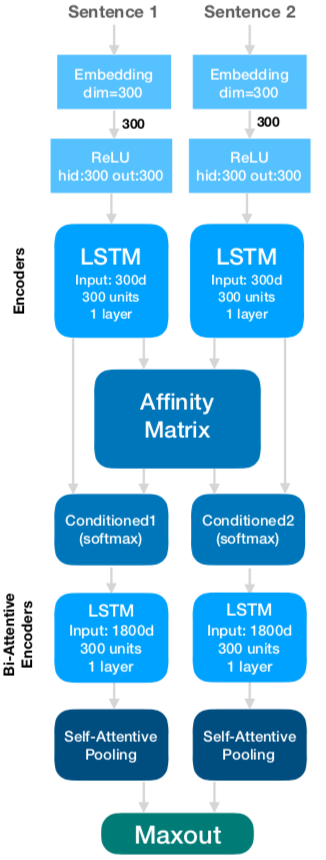
\includegraphics[scale=0.5]{images/arch_standard.png}
	\caption{Architecture for bi-attentive classification network.}
\end{figure}


The basic architecture was augmented by using part of speech (POS) tags as features. Given enough data, the LSTM should be able to learn sequence-to-sequence relationships and implicitly learn parts of speech and their importance. However, the motivation for using POS tags as an additional feature came from observing the way humans learn. For example, adjectives carry a lot of weight with regards to sentiment, but they cannot be taken alone. They must be considered in context as parts of a greater structure. Knowledge of their presence and their POS can indicate a more important structure. The expectation was that by adding explicitly POS tags, the model would be able to more quickly learn which structures are important and which are not. 

\begin{figure}[H]
	%\centering
	%	\captionsetup{justification=centering}
	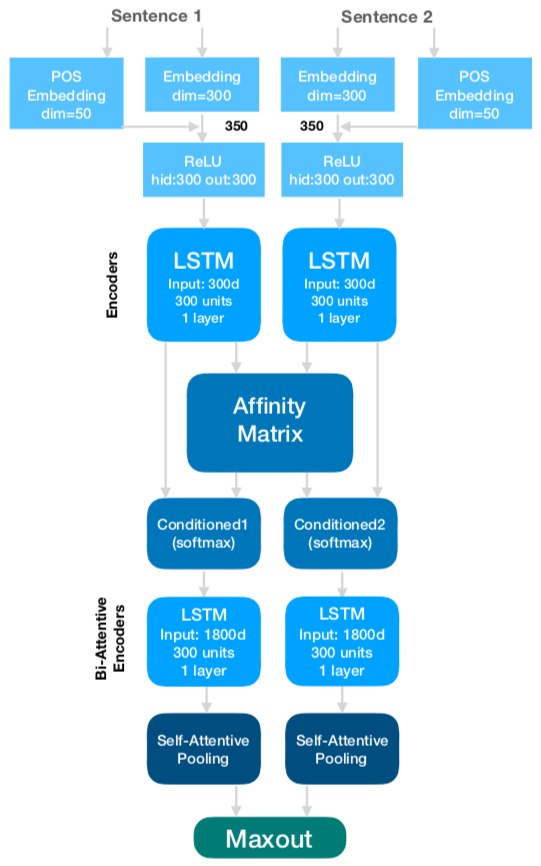
\includegraphics[width=0.5\textwidth]{images/arch_modified.png}
	\caption{Architecture for bi-attentive classification network with part of speech as a feature.}
\end{figure}

The above below shows how this modification was implemented. NLTK tagger was used to tag tokens into one of 37 possible tags, with tags 1-36 being the standard Penn Treebank tags and tag 37 being <unk>. The POS embedding weights were randomly initialized using Xavier initialization \cite{glorot_bengio} and then updated via backpropagation during training time. The POS embedding vector is then concatenated to the word embedding vector before being passed through the ReLU layer. The downstream parts of the network are the exact same in both instances.

\subsubsection{\textbf{Loss Weighting}}
When training data exhibits severe class imbalances, such as in the case of the RecSys2013 dataset, a model will "learn" to output the most probable class without actually building an expressive and generalizable mapping from input feature space to output classes. One technique to solve this is loss weighting, wherein a penalty is multiplied backward in the network to adjust weights. Classes with more members are penalized by multiplying their weights with a smaller number to keep overall weight magnitude relatively lower. Classes with fewer members are penalized significantly less or not at all. The downside of this method is that training time increases as the weights are rescaled at each iteration. There are two simple ways of doing loss weighting:
\begin{enumerate}
	\item \textbf{Inverse Class Size} In this method, the weighting vector is created by iterating through each class, finding the total number of examples in the class, and then inverting this value. For example, if the class:size distribution were as follows: {1:10, 2:10, 3:5, 4:50, 5:25}, then the weighting vector would be:
	\begin{equation}
	weights = [\frac{1}{10}, \frac{1}{10}, \frac{1}{5}, \frac{1}{50}, \frac{1}{25}]
	\end{equation}
	
	\item \textbf{Inverse Probability}  In this method, the weighting vector is created by iterating through each class, finding the total number of examples in the class, dividing each instance by the total number of examples in the entire set, and then taking the inverse probability by subtracting this value from 1. Taking the same distribution from before, the raw class probabilities are:
	\begin{equation}
	raw\_probabilities = [\frac{10}{100}, \frac{10}{100}, \frac{5}{100}, \frac{50}{100}, \frac{25}{100}]
	\end{equation}
	After subtracting each term from 1 to take the inverse, the weighting vector is:
	\begin{equation}
	weights = [\frac{90}{100}, \frac{90}{100}, \frac{95}{100}, \frac{50}{100}, \frac{75}{100}]
	\end{equation}
\end{enumerate}
In both cases, the smallest class (class 3) is penalized the least amount. The largest class (class 4) is penalized the most. However, the penalization is much larger in method 1. Method 2 was used instead in order to balance the weighting with training speed.

\section{Approach}
The approach was to train two main sets of models in addition to the baseline models. In the following descriptions, the balanced sets come from the Yelp full dataset and the imbalanced sets come from the RecSys2013 dataset. Performance metrics include raw accuracy, F1-score, mean-squared error, and a confusion matrix. Mean-squared error gives us an indicator of how close the model predictions were to ground truth, and is applicable here due to the inherent ambiguity between the subsets within the low and high rating categories.
\par 
Evaluation on the balanced dataset will provide an indicator of overall classifier performance. Evaluation on the imbalanced dataset and analysis of the corresponding confusion matrices will test how effectively the model learned the implicit mapping between sentiment and star rating. A model that has effectively learned this mapping should not only have a saturated diagonal in the confusion matrix, but also relatively balanced F1-scores for each class.

\subsection{Baseline Models}
The random forest and feed-forward neural network models were partitioned into two sets: trained \& tested on balanced data as well as trained \& tested on imbalanced data.  


\subsection{Set 1: Models Trained on Balanced Data}
The first set of models were trained on the balanced dataset and tested on both a balanced and imbalanced test set. Since all models in the first set were trained on balanced data, none of these models were run with the loss weighting mechanism. There were six configurations of this first set, each with a single variation on the control model. The control model was trained with no POS features, pre-trained embeddings without weight updates, and no limit on vocabulary size. These configurations are summarized in Table \ref{tab:set1_exp}. Model 2's configuration included training word embeddings on the full vocab size, but this model was not trained because of the memory requirements. Similarly, model 5 involved training both POS embeddings and word embeddings, but was not run due to memory requirements.
\begin{table*}[ht]
	\centering
	\begin{tabular}{|c|c|c|c|c|c|c|c|}
		\hline
		Model & Training Set & Testing Set 1 & Testing Set 2 & Loss Weighting  & POS & Custom Embeddings & Max Words \\
		\hline
		1 & Balanced & Balanced & Imbalanced & No & No & No & All \\
		3 & Balanced & Balanced & Imbalanced & No & Yes & No & All \\
		5 & Balanced & Balanced & Imbalanced & No & No & No & 80000  \\
		6 & Balanced & Balanced & Imbalanced & No & No & Yes & 80000 \\
		7 & Balanced & Balanced & Imbalanced & No & Yes & No & 80000 \\
		8 & Balanced & Balanced & Imbalanced & No & Yes & Yes & 80000 \\
		\hline
	\end{tabular}
	\caption{\label{tab:set1_exp}Model configurations for set 1.}
\end{table*}

\subsection{Set 2: Models Trained on Imbalanced Data}
The second set of models were trained on the imbalanced data and tested on both a balanced and imbalanced test set. There were nine configurations of this second set. The control model was run with no loss weighting, no POS features, pre-trained embeddings without weight updates, and no limit on vocabulary size. 
\begin{table*}[ht]
	\centering
	\begin{tabular}{|c|c|c|c|c|c|c|c|}
		\hline
		Model & Training Set & Testing Set 1 & Testing Set 2 & Loss Weighting  & POS & Custom Embeddings & Max Words \\
		\hline
		9  & Imbalanced & Balanced & Imbalanced & No  & No & No & All \\
		10 & Imbalanced & Balanced & Imbalanced & Yes & No & No & All \\
		11 & Imbalanced & Balanced & Imbalanced & Yes & No & Yes & All  \\
		12 & Imbalanced & Balanced & Imbalanced & Yes & Yes & No & All \\
		13 & Imbalanced & Balanced & Imbalanced & Yes & Yes & Yes & All \\
		14 & Imbalanced & Balanced & Imbalanced & Yes & No & No & 80000 \\
		15 & Imbalanced & Balanced & Imbalanced & Yes & No & Yes & 80000 \\
		16 & Imbalanced & Balanced & Imbalanced & Yes & Yes & No & 80000 \\
		17 & Imbalanced & Balanced & Imbalanced & Yes & Yes & Yes & 80000 \\
		\hline
	\end{tabular}
	\caption{\label{tab:set2_exp}Model configurations for set 2.}
\end{table*}

\subsection{Hypotheses}
There were several hypotheses, summarized below:
\begin{enumerate}
	\item Limiting the vocab size to the top 80,000-100,000 or so frequent words would not drastically reduce classification performance, while at the same time reducing training time.
	\item Part of speech features will result in higher classification performance and potentially faster training time.
	\item Training word embeddings on the specific training corpus will increase classifier performance.
	\item Loss weighting will improve classifier performance and result in more diagonal entries in the confusion matrices.
\end{enumerate}

\section{Results}
The full set of results across all models and all metrics can be found in the console output dumps on the project GitHub. Core metrics for the self-attentive classifier, such as accuracy, F1, and MSE are shown in tables \ref{tab:resset1_exp} and \ref{tab:resset2_exp}. Recall that models 1-8 were trained on balanced data and models 9-17 were trained on imbalanced data. 
\subsection{Baseline Models}
Table \ref{tab:baselines_imbalanced} shows the results for the baseline models trained on the imbalanced dataset and tested on a held out portion of data from the imbalanced dataset. Since there are 79708 examples in class 4 and a total of 229898 examples, and since the testing set has nearly the same class proportion as the training set, a model could simply output class 4 and achieve 34.67\% accuracy. F1 score would be low. Since most examples are grouped into classes 4 and 5, a model outputting primarily 4 or 5 would not have terribly high MSE. In fact, the models trained and tested on the imbalanced dataset show a relatively lower MSE than those trained and tested on the balanced dataset for this very reason. Thus, MSE is not the most effective metric when studying results of models trained \& tested on the imbalanced dataset. The neural network model achieved better accuracy, F1 score, and MSE. 

\begin{table}[H]
	\begin{tabular}{|c|c|c|c|}
		\hline
		\textbf{Model}    & \textbf{Accuracy} & \textbf{F1 Score} & \textbf{MSE} \\ \hline
		Random Forest     & 37.94\%           & 0.2088            & 1.5352       \\
		FF Neural Network & 39.79\%           & 0.3241            & 1.4241    \\ \hline
	\end{tabular}
	\caption{\label{tab:baselines_imbalanced} Results for baseline models trained \& tested on the imbalanced dataset.}
\end{table}
Table \ref{tab:baselines_balanced} shows the results for the baseline models trained on the balanced dataset and tested on a held out portion of data from the balanced dataset. In this case, it's much more difficult to achieve a low MSE because of the perfectly balanced data. A low MSE would indicate that the model is outputting class predictions close to their true value. Since the data is balanced, MSE is an effective metric here. One again, the neural network performed better than the random forest in all metrics. Both models show lower accuracy than in \ref{tab:baselines_imbalanced} because the data is balanced, thus the model cannot "learn" to output a high probability class. The F1 scores of both models were higher, indicating that training on the balanced dataset allowed the models to learn the mapping from text features to rating more effectively.

\begin{table}[H]
	\begin{tabular}{|c|c|c|c|}
		\hline
		\textbf{Model}    & \textbf{Accuracy} & \textbf{F1 Score} & \textbf{MSE} \\ \hline
		Random Forest     & 30.94\%           & 0.3014            & 3.1237       \\
		FF Neural Network & 35.17\%           & 0.3402            & 2.6607    \\ \hline
	\end{tabular}
	\caption{\label{tab:baselines_balanced} Results for baseline models trained \& tested on the balanced dataset.}
\end{table}


\subsection{Set 1}
The first point of comparison would be between a model trained with pre-trained embeddings vs. one with embeddings trained at each iteration. This comparison could not be done with the full vocab size. Given the models that were trained with the full vocab size, the question to be answered is the effect of POS tags as a feature on model performance. Interestingly enough, model 3 (with POS features) performed worse in accuracy, overall F1-score, and MSE than model 1 for both balanced and imbalanced evaluation sets. However, model 3 boasted higher F1-scores for minority classes in both balanced and imbalanced evaluations.
\par 
The next expectation was that limiting the vocab size to the 80,000 most frequent words would not drastically reduce classifier performance while significantly improving training time. This was confirmed and can be shown in the comparison of performance between models 1 and 5. In fact, model 5 narrowly outperformed model 1 in terms of mean-squared error for evaluation on the balanced dataset, scoring 0.59912 vs. 0.60518. Model 5's minority class F1-scores were also marginally better than model 1's scores.  Performance of model 5 was slightly worse than model 1 on the imbalanced dataset for all categories, including minority class F1-score.
\par 
Another expectation was that training word embeddings would increase classifier performance. Model 6's word embeddings were trained whereas model 5 used the pre-trained GloVe embeddings. Model 6 outperformed model 5 in every single evaluation metric, for both balanced and imbalanced evaluation sets.
\par 
Both model 7 and model 8 had a vocab size of 80,000, but model 7 used POS features and pre-trained embeddings whereas model 8 uses both POS features and trains its embeddings. Model 7's performance is worse across the board than model 6, but model 8 outperforms both of them.
\par 
Of set 1, model 8 performed the best with model 6 performing second best. 

\begin{table}[H]
	\begin{tabular}{|c|c|c|c|}
		\hline
		\textbf{Model} & \textbf{Accuracy} & \textbf{F1 Score} & \textbf{MSE} \\ \hline
		1              & 64.52\%             &  0.6396\%        &  0.6051   \\
		3              & 63.67\%             &  0.6347\%        &  0.6155   \\
		5              & 64.48\%             &  0.6393\%        &  0.5991   \\
		6              & 65.68\%             &  0.6586\%        &  0.4868   \\
		7              & 63.75\%             &  0.6343\%        &  0.6239   \\
		8              & 66.01\%             &  0.6589\%        &  0.5012   \\
		9              & 60.51\%             &  0.6011\%        &  0.7021   \\
		10             & 60.46\%             &  0.6022\%        &  0.7139   \\
		11             & 59.68\%             &  0.5874\%        &  0.6548   \\
		12             & 59.05\%             &  0.5845\%        &  0.7440   \\	
		13             & 59.93\%             &  0.5953\%        &  0.6812   \\	
		14             & 59.23\%             &  0.5914\%        &  0.7391   \\	
		15             & 59.23\%             &  0.5804\%        &  0.6913   \\	
		16             & 60.35\%             &  0.6044\%        &  0.6685   \\	
		17             & 59.55\%             &  0.5855\%        &  0.7030   \\ \hline	
	\end{tabular}
	\caption{\label{tab:resset1_exp}Results for set 1: Models tested on balanced data.}
\end{table}

\subsection{Set 2}
The first step was to determine if loss weighting via inverse probability is effective enough to mitigate a severe class imbalance problem. Model 9 does not use loss weighting while model 10 does. The loss weighting marginally improves the F1-scores of minority classes 2 and 3 (corresponding to 2 star and 3 star ratings), but every other metric decreases by a small amount. Despite only this small improvement, loss weighting was used for the remainder of the experiments involving training on the imbalanced set.
\par 
Models 10 and 12 differ only in the introduction of POS features. Both use the full vocab of the imbalanced dataset. The results here further support the results from set 1: adding POS features to a model training on a full-sized vocab without training word embeddings reduces performance across all categories. However, in this situation, minority class F1-scores did not improve.
\par 
Models 9 and 14 differ in maximum vocab size. Models 14-17 are limited to the 80,000 most frequent words. The results here also support hypothesis 1 and the results obtained from set 1: limiting vocab size marginally reduces performance while decreasing training time. Model 9 performed worse in every category but each difference was less than $1\%$.
\par 
When trained on the imbalanced dataset with vocab limit, adding in POS features actually improved performance in nearly every way, with the exception of a small MSE increase for the imbalanced evaluation set. Unlike set 1, the best performance was not exhibited by a combination of POS features and trained embeddings on the limited vocab size, but rather by just adding POS features and training on the limited vocab size. The best performing model from this set was model 16.
\begin{table}[H]
	\begin{tabular}{|c|c|c|c|}
		\hline
		\textbf{Model} & \textbf{Accuracy} & \textbf{F1 Score} & \textbf{MSE} \\ \hline
		1              & 61.41\%             &  0.6084\%        &  0.7177   \\
		3              & 59.60\%             &  0.5960\%        &  0.8505   \\
		5              & 60.53\%             &  0.6053\%        &  0.7823   \\
		6              & 61.50\%             &  0.6150\%        &  0.6078   \\
		7              & 60.02\%             &  0.6002\%        &  0.7792   \\
		8              & 62.27\%             &  0.6227\%        &  0.6461   \\
		9              & 59.41\%             &  0.5941\%        &  0.8562   \\
		10             & 58.93\%             &  0.5893\%        &  0.8994   \\
		11             & 55.44\%             &  0.5544\%        &  0.9317   \\
		12             & 57.82\%             &  0.5782\%        &  0.8735   \\	
		13             & 59.28\%             &  0.5928\%        &  0.7899   \\	
		14             & 59.70\%             &  0.5970\%        &  0.7902   \\	
		15             & 53.35\%             &  0.5335\%        &  1.0368   \\	
		16             & 60.25\%             &  0.6025\%        &  0.8011   \\	
		17             & 57.16\%             &  0.5716\%        &  0.8531   \\ \hline	
	\end{tabular}
	\caption{\label{tab:resset2_exp}Results for set 2: Models tested on imbalanced data.}
\end{table}

\section{Discussion}
Due to ambiguity and some blurred lines between the classes, mean-squared error in conjunction with F1-score proved to be a good evaluation metric. The self-attentive classifier labeled the negative Armando's review (discussed in the introduction) as 1-star, whereas the ground truth was 3 star. This, combined with the performance increases across all metrics when compared to the baselines suggests that the model was able to learn a basic bijection between the text features and the star rating. However, it's worth noting that ambiguity does not exist only at the extremes. For example, here is a 3 star review that the self-attentive classifier labeled as a 4-star review:
\begin{quote}
	"I went to Z Tejas with a bunch of people (about 25) last night.  We had a great experience from start to finish.  At the beginning my lady and I were early so the waiter got us our drinks and continued to make sure we were good to go.  We wanted to wait for our friends so food wasn't necessary at this time, but the drinks were flowing and the waiter (Jeff) was very cool, friendly, and down to earth.  All of our friends showed up and we let the good times roll.  Chips and salsa, drinks, water, and the delicious cornbread, they all came very fast and it didn't take any begging on our part.  I got a chicken dish which was really good, I stuffed myself silly.  My lady got a side salad which was huge, she couldn't even finish it and she said it was really good.  Oh! and the food came fast by the way (surprising when you have 25 people.The overall vibe of the place is really cool, very trendy and fancy but reasonable prices.  Big screens everywhere, gotta love that since there were some great College FB games on last night.  Great experience, thanks Jeff \& Z Tejas."
\end{quote}
This review has many positive words and phrases: cool, friendly, 'down to earth', delicious, 'very trendy', 'great experience'. This could pass as a higher rated review, and the classifier has chosen to assign a higher value. Without MSE, this example would be considered a complete misclassification, and there would be no notion of "closeness".
 
\subsection{Hypothesis 1}
As expected, limiting the vocab size to the 80,000 most frequent words did not drastically reduce classifier performance. In some instances, performance was actually increased. Training time was reduced by several hours. 

\subsection{Hypothesis 2}
While adding POS tags as a feature did not significantly improve performance across the metrics defined, it did result in an interesting performance boost in terms of training time. The following figure plots the training and validation accuracies across three epochs for models 5 and 7. Both models have vocab limited to 80,000 words. Model 7 uses POS features whereas model 5 does not. The plot below shows that model 7 (blue) trains significantly faster than model 5 (red). In these early epochs, overfitting is not as much of an issue and the validation accuracies track both training curves well.
\begin{figure}[H]
	%\centering
	%	\captionsetup{justification=centering}
	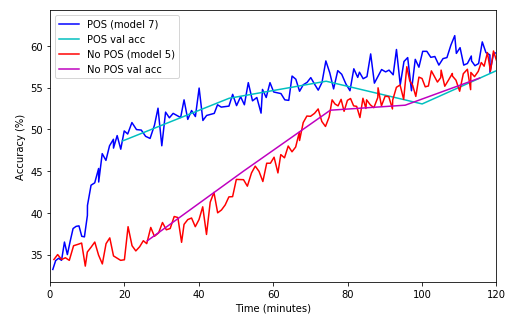
\includegraphics[width=0.5\textwidth]{images/training_speed.png}
	\caption{A comparison of training speed and validation accuracy for models 5 and 7.}
\end{figure}
These models both saturated in terms of validation accuracy. However, model 7 reached this saturation point nearly an hour before model 5. At the 120 minute mark, model 5's training and validation accuracy finally intersect those of model 7.
\par 
Across the board, the POS features did not dramatically improve classifier performance metrics but they did reduce the time it takes to reach a saturation point in training. Since this is a sentiment analysis task, the POS tagging may not be extremely useful for determining class since both positive and negative sentiment can be related to the same tag. One example might be the words "delicious" and "horrible". In terms of sentiment, these belong in different classes, but they share the same POS tag. During training, explicitly showing the model the POS tags and training this embedding layer may help the model learn where to look but it does not show the model the underlying meaning of the structure or word.

\subsection{Hypothesis 3}
In general, training word embeddings on the specific training corpus marginally increased classifier performance when coupled with a vocab limited to the most frequent words.

\subsection{Hypothesis 4}
Inverse probability loss weighting provided marginal improvement in the minority class F1-scores for the imbalanced data, namely the 1, 2, and 3 star review categories. Other metrics were not improved and some worsened, likely due to the impact penalization has in terms of how quickly the model can learn. A more significant penalization like inverting the class size may improve classifier performance on such an imbalanced dataset.

\section{Conclusion}
Measurable results were found for all four hypothesis. It was shown that limiting vocab size is an effective way to maintain model performance while drastically speeding up training time. While the initial hypothesis was that POS tags would allow for better classification performance and potentially faster training time, only the latter was true. Models trained with POS features trained faster but did not gain any expressiveness over models trained without POS tags. Both models' training and validation accuracies intersected after about two hours of training time, after which performance was relatively equal. It was found that training custom word embeddings improved performance, but not drastically. Inverse probability loss penalization was used to deal with the class imbalance of the recsys dataset, but this proved to be ineffective due to how severe the imbalance was. A more significant penalization should be attem 

\begin{acks}
I would like to thank Wasi Ahmad for his continuous patience, guidance, and regular assistance with issues during this project. I'd also like to thank Rizwan Parvez for providing high level direction, advice, and some early on assistance. I'm grateful to Professor Kai-Wei Chang for also providing direction and motivation for the project.

\end{acks}


% jteoh start of original sample that I didn't simply replace
% This contains a bunch of things, including appendix examples

% \section{The Body of The Paper}
% Typically, the body of a paper is organized into a hierarchical
% structure, with numbered or unnumbered headings for sections,
% subsections, sub-subsections, and even smaller sections.  The command
% \texttt{{\char'134}section} that precedes this paragraph is part ofDownload



% such a hierarchy.\



% numbering and placement of these headings for you, when you use the
% appropriate heading commands around the titles of the headings.  If
% you want a sub-subsection or smaller part to be unnumbered in your
% output, simply append an asterisk to the command name.  Examples of
% both numbered and unnumbered headings will appear throughout the
% balance of this sample document.

% Because the entire article is contained in the \textbf{document}
% environment, you can indicate the start of a new paragraph with a
% blank line in your input file; that is why this sentence forms a
% separate paragraph.

% \subsection{Type Changes and {\itshape Special} Characters}

% We have already seen several typeface changes in this sample.  You can
% indicate italicized words or phrases in your text with the command
% \texttt{{\char'134}textit}; emboldening with the command
% \texttt{{\char'134}textbf} and typewriter-style (for instance, for
% computer code) with \texttt{{\char'134}texttt}.  But remember, you do
% not have to indicate typestyle changes when such changes are part of
% the \textit{structural} elements of your article; for instance, the
% heading of this subsection will be in a sans serif\footnote{Another
%   footnote here.  Let's make this a rather long one to see how it
%   looks.} typeface, but that is handled by the document class file.
% Take care with the use of\footnote{Another footnote.}  the
% curly braces in typeface changes; they mark the beginning and end of
% the text that is to be in the different typeface.

% You can use whatever symbols, accented characters, or non-English
% characters you need anywhere in your document; you can find a complete
% list of what is available in the \textit{\LaTeX\ User's Guide}
% \cite{Lamport:LaTeX}.

% \subsection{Math Equations}
% You may want to display math equations in three distinct styles:
% inline, numbered or non-numbered display.  Each of
% the three are discussed in the next sections.

% \subsubsection{Inline (In-text) Equations}
% A formula that appears in the running text is called an
% inline or in-text formula.  It is produced by the
% \textbf{math} environment, which can be
% invoked with the usual \texttt{{\char'134}begin\,\ldots{\char'134}end}
% construction or with the short form \texttt{\$\,\ldots\$}. You
% can use any of the symbols and structures,
% from $\alpha$ to $\omega$, available in
% \LaTeX~\cite{Lamport:LaTeX}; this section will simply show a
% few examples of in-text equations in context. Notice how
% this equation:
% \begin{math}
%   \lim_{n\rightarrow \infty}x=0
% \end{math},
% set here in in-line math style, looks slightly different when
% set in display style.  (See next section).

% \subsubsection{Display Equations}
% A numbered display equation---one set off by vertical space from the
% text and centered horizontally---is produced by the \textbf{equation}
% environment. An unnumbered display equation is produced by the
% \textbf{displaymath} environment.

% Again, in either environment, you can use any of the symbols
% and structures available in \LaTeX\@; this section will just
% give a couple of examples of display equations in context.
% First, consider the equation, shown as an inline equation above:
% \begin{equation}
%   \lim_{n\rightarrow \infty}x=0
% \end{equation}
% Notice how it is formatted somewhat differently in
% the \textbf{displaymath}
% environment.  Now, we'll enter an unnumbered equation:
% \begin{displaymath}
%   \sum_{i=0}^{\infty} x + 1
% \end{displaymath}
% and follow it with another numbered equation:
% \begin{equation}
%   \sum_{i=0}^{\infty}x_i=\int_{0}^{\pi+2} f
% \end{equation}
% just to demonstrate \LaTeX's able handling of numbering.

% \subsection{Citations}
% Citations to articles~\cite{bowman:reasoning,
% clark:pct, braams:babel, herlihy:methodology},
% conference proceedings~\cite{clark:pct} or maybe
% books \cite{Lamport:LaTeX, salas:calculus} listed
% in the Bibliography section of your
% article will occur throughout the text of your article.
% You should use BibTeX to automatically produce this bibliography;
% you simply need to insert one of several citation commands with
% a key of the item cited in the proper location in
% the \texttt{.tex} file~\cite{Lamport:LaTeX}.
% The key is a short reference you invent to uniquely
% identify each work; in this sample document, the key is
% the first author's surname and a
% word from the title.  This identifying key is included
% with each item in the \texttt{.bib} file for your article.

% The details of the construction of the \texttt{.bib} file
% are beyond the scope of this sample document, but more
% information can be found in the \textit{Author's Guide},
% and exhaustive details in the \textit{\LaTeX\ User's
% Guide} by Lamport~\shortcite{Lamport:LaTeX}.

% This article shows only the plainest form
% of the citation command, using \texttt{{\char'134}cite}.

% Some examples.  A paginated journal article \cite{Abril07}, an enumerated
% journal article \cite{Cohen07}, a reference to an entire issue \cite{JCohen96},
% a monograph (whole book) \cite{Kosiur01}, a monograph/whole book in a series (see 2a in spec. document)
% \cite{Harel79}, a divisible-book such as an anthology or compilation \cite{Editor00}
% followed by the same example, however we only output the series if the volume number is given
% \cite{Editor00a} (so Editor00a's series should NOT be present since it has no vol. no.),
% a chapter in a divisible book \cite{Spector90}, a chapter in a divisible book
% in a series \cite{Douglass98}, a multi-volume work as book \cite{Knuth97},
% an article in a proceedings (of a conference, symposium, workshop for example)
% (paginated proceedings article) \cite{Andler79}, a proceedings article
% with all possible elements \cite{Smith10}, an example of an enumerated
% proceedings article \cite{VanGundy07},
% an informally published work \cite{Harel78}, a doctoral dissertation \cite{Clarkson85},
% a master's thesis: \cite{anisi03}, an online document / world wide web
% resource \cite{Thornburg01, Ablamowicz07, Poker06}, a video game (Case 1) \cite{Obama08} and (Case 2) \cite{Novak03}
% and \cite{Lee05} and (Case 3) a patent \cite{JoeScientist001},
% work accepted for publication \cite{rous08}, 'YYYYb'-test for prolific author
% \cite{SaeediMEJ10} and \cite{SaeediJETC10}. Other cites might contain
% 'duplicate' DOI and URLs (some SIAM articles) \cite{Kirschmer:2010:AEI:1958016.1958018}.
% Boris / Barbara Beeton: multi-volume works as books
% \cite{MR781536} and \cite{MR781537}.

% A couple of citations with DOIs: \cite{2004:ITE:1009386.1010128,
%   Kirschmer:2010:AEI:1958016.1958018}.

% Online citations: \cite{TUGInstmem, Thornburg01, CTANacmart}.


% \subsection{Tables}
% Because tables cannot be split across pages, the best
% placement for them is typically the top of the page
% nearest their initial cite.  To
% ensure this proper ``floating'' placement of tables, use the
% environment \textbf{table} to enclose the table's contents and
% the table caption.  The contents of the table itself must go
% in the \textbf{tabular} environment, to
% be aligned properly in rows and columns, with the desired
% horizontal and vertical rules.  Again, detailed instructions
% on \textbf{tabular} material
% are found in the \textit{\LaTeX\ User's Guide}.

% Immediately following this sentence is the point at which
% Table~\ref{tab:freq} is included in the input file; compare the
% placement of the table here with the table in the printed
% output of this document.

% \begin{table}
%   \caption{Frequency of Special Characters}
%   \label{tab:freq}
%   \begin{tabular}{ccl}
%     \toprule
%     Non-English or Math&Frequency&Comments\\
%     \midrule
%     \O & 1 in 1,000& For Swedish names\\
%     $\pi$ & 1 in 5& Common in math\\
%     \$ & 4 in 5 & Used in business\\
%     $\Psi^2_1$ & 1 in 40,000& Unexplained usage\\
%   \bottomrule
% \end{tabular}
% \end{table}

% To set a wider table, which takes up the whole width of the page's
% live area, use the environment \textbf{table*} to enclose the table's
% contents and the table caption.  As with a single-column table, this
% wide table will ``float'' to a location deemed more desirable.
% Immediately following this sentence is the point at which
% Table~\ref{tab:commands} is included in the input file; again, it is
% instructive to compare the placement of the table here with the table
% in the printed output of this document.


% \begin{table*}
%   \caption{Some Typical Commands}
%   \label{tab:commands}
%   \begin{tabular}{ccl}
%     \toprule
%     Command &A Number & Comments\\
%     \midrule
%     \texttt{{\char'134}author} & 100& Author \\
%     \texttt{{\char'134}table}& 300 & For tables\\
%     \texttt{{\char'134}table*}& 400& For wider tables\\
%     \bottomrule
%   \end{tabular}
% \end{table*}
% % end the environment with {table*}, NOTE not {table}!

% It is strongly recommended to use the package booktabs~\cite{Fear05}
% and follow its main principles of typography with respect to tables:
% \begin{enumerate}
% \item Never, ever use vertical rules.
% \item Never use double rules.
% \end{enumerate}
% It is also a good idea not to overuse horizontal rules.


% \subsection{Figures}

% Like tables, figures cannot be split across pages; the best placement
% for them is typically the top or the bottom of the page nearest their
% initial cite.  To ensure this proper ``floating'' placement of
% figures, use the environment \textbf{figure} to enclose the figure and
% its caption.

% This sample document contains examples of \texttt{.eps} files to be
% displayable with \LaTeX.  If you work with pdf\LaTeX, use files in the
% \texttt{.pdf} format.  Note that most modern \TeX\ systems will convert
% \texttt{.eps} to \texttt{.pdf} for you on the fly.  More details on
% each of these are found in the \textit{Author's Guide}.

% \begin{figure}
% 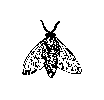
\includegraphics{fly}
% \caption{A sample black and white graphic.}
% \end{figure}

% \begin{figure}
% 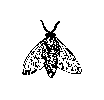
\includegraphics[height=1in, width=1in]{fly}
% \caption{A sample black and white graphic
% that has been resized with the \texttt{includegraphics} command.}
% \end{figure}


% As was the case with tables, you may want a figure that spans two
% columns.  To do this, and still to ensure proper ``floating''
% placement of tables, use the environment \textbf{figure*} to enclose
% the figure and its caption.  And don't forget to end the environment
% with \textbf{figure*}, not \textbf{figure}!

% \begin{figure*}
% 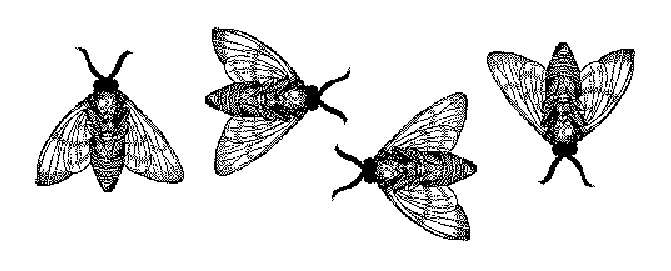
\includegraphics{flies}
% \caption{A sample black and white graphic
% that needs to span two columns of text.}
% \end{figure*}


% \begin{figure}
% 
\includegraphics[height=1in, width=1in]{rosette}
% \caption{A sample black and white graphic that has
% been resized with the \texttt{includegraphics} command.}
% \end{figure}

% \subsection{Theorem-like Constructs}

% Other common constructs that may occur in your article are the forms
% for logical constructs like theorems, axioms, corollaries and proofs.
% ACM uses two types of these constructs:  theorem-like and
% definition-like.

% Here is a theorem:
% \begin{theorem}
%   Let $f$ be continuous on $[a,b]$.  If $G$ is
%   an antiderivative for $f$ on $[a,b]$, then
%   \begin{displaymath}
%     \int^b_af(t)\,dt = G(b) - G(a).
%   \end{displaymath}
% \end{theorem}

% Here is a definition:
% \begin{definition}
%   If $z$ is irrational, then by $e^z$ we mean the
%   unique number that has
%   logarithm $z$:
%   \begin{displaymath}
%     \log e^z = z.
%   \end{displaymath}
% \end{definition}

% The pre-defined theorem-like constructs are \textbf{theorem},
% \textbf{conjecture}, \textbf{proposition}, \textbf{lemma} and
% \textbf{corollary}.  The pre-defined de\-fi\-ni\-ti\-on-like constructs are
% \textbf{example} and \textbf{definition}.  You can add your own
% constructs using the \textsl{amsthm} interface~\cite{Amsthm15}.  The
% styles used in the \verb|\theoremstyle| command are \textbf{acmplain}
% and \textbf{acmdefinition}.

% Another construct is \textbf{proof}, for example,

% \begin{proof}
%   Suppose on the contrary there exists a real number $L$ such that
%   \begin{displaymath}
%     \lim_{x\rightarrow\infty} \frac{f(x)}{g(x)} = L.
%   \end{displaymath}
%   Then
%   \begin{displaymath}
%     l=\lim_{x\rightarrow c} f(x)
%     = \lim_{x\rightarrow c}
%     \left[ g{x} \cdot \frac{f(x)}{g(x)} \right ]
%     = \lim_{x\rightarrow c} g(x) \cdot \lim_{x\rightarrow c}
%     \frac{f(x)}{g(x)} = 0\cdot L = 0,
%   \end{displaymath}
%   which contradicts our assumption that $l\neq 0$.
% \end{proof}

% \section{Conclusions}
% This paragraph will end the body of this sample document.
% Remember that you might still have Acknowledgments or
% Appendices; brief samples of these
% follow.  There is still the Bibliography to deal with; and
% we will make a disclaimer about that here: with the exception
% of the reference to the \LaTeX\ book, the citations in
% this paper are to articles which have nothing to
% do with the present subject and are used as
% examples only.
% %\end{document}  % This is where a 'short' article might terminate



% \appendix
% %Appendix A
% \section{Headings in Appendices}
% The rules about hierarchical headings discussed above for
% the body of the article are different in the appendices.
% In the \textbf{appendix} environment, the command
% \textbf{section} is used to
% indicate the start of each Appendix, with alphabetic order
% designation (i.e., the first is A, the second B, etc.) and
% a title (if you include one).  So, if you need
% hierarchical structure
% \textit{within} an Appendix, start with \textbf{subsection} as the
% highest level. Here is an outline of the body of this
% document in Appendix-appropriate form:
% \subsection{Introduction}
% \subsection{The Body of the Paper}
% \subsubsection{Type Changes and  Special Characters}
% \subsubsection{Math Equations}
% \paragraph{Inline (In-text) Equations}
% \paragraph{Display Equations}
% \subsubsection{Citations}
% \subsubsection{Tables}
% \subsubsection{Figures}
% \subsubsection{Theorem-like Constructs}
% \subsubsection*{A Caveat for the \TeX\ Expert}
% \subsection{Conclusions}
% \subsection{References}
% Generated by bibtex from your \texttt{.bib} file.  Run latex,
% then bibtex, then latex twice (to resolve references)
% to create the \texttt{.bbl} file.  Insert that \texttt{.bbl}
% file into the \texttt{.tex} source file and comment out
% the command \texttt{{\char'134}thebibliography}.
% % This next section command marks the start of
% % Appendix B, and does not continue the present hierarchy
% \section{More Help for the Hardy}

% Of course, reading the source code is always useful.  The file
% \path{acmart.pdf} contains both the user guide and the commented
% code.

% \begin{acks}
%   The authors would like to thank Dr. Yuhua Li for providing the
%   MATLAB code of the \textit{BEPS} method.

%   The authors would also like to thank the anonymous referees for
%   their valuable comments and helpful suggestions. The work is
%   supported by the \grantsponsor{GS501100001809}{National Natural
%     Science Foundation of
%     China}{http://dx.doi.org/10.13039/501100001809} under Grant
%   No.:~\grantnum{GS501100001809}{61273304}
%   and~\grantnum[http://www.nnsf.cn/youngscientists]{GS501100001809}{Young
%     Scientists' Support Program}.

% \end{acks}



\bibliographystyle{ACM-Reference-Format}
\bibliography{report-bibliography-acm}

\appendix
\section*{APPENDIX}
  \section{Source code}
    https://github.com/jdhurwitz/pyfinder/blob/master/README.md
    
\end{document}
